%______________________________________________________________________________
%************************* HEADER *********************************************
\documentclass[]{scrreprt}
		
    
\usepackage{a4}
\usepackage[T1]{fontenc}
\usepackage[utf8]{inputenc}
\usepackage{lmodern}

\usepackage{subfigure}
\usepackage{epsfig}
\usepackage{graphicx}
\usepackage{graphics}
% \usepackage{array}
% \usepackage{units}
%\usepackage{cite}	 % Für Bibtex
\usepackage[noadjust]{cite}	 % Für Bibtex, noadjust: Keine Leerzeichen vor Referenz _[X]
\usepackage[]{placeins}  % für \FloatBarrier
\usepackage{amssymb} 
\usepackage[]{amsmath}   % Formelumgebung für begin{align]
% \usepackage{longtable}   % Mehrseitige Tabellen (Symbole)
\usepackage{booktabs}    % horizontale Linien in Tabellen
\usepackage{wrapfig}
\usepackage{scrhack}     % prevent warning for the following 'listings'
\usepackage{listings}    % Für Quellcode einbinden
\usepackage[onehalfspacing]{setspace}   % Einfacher Zeilenabstand für Tabellen
\usepackage{tabularx}

% \usepackage{tocbasic}
\usepackage[pdfpagelabels, plainpages=false]{hyperref} 
% \usepackage[linktocpage,pdfborderstyle={/S/U/W 1}]{hyperref}  % Links nur unterstrichen, nicht umrandet




% ---------------- header ----------------------
\usepackage{scrlayer-scrpage}
\automark{chapter}
\automark*{section}
\clearpairofpagestyles
\ihead{\headmark}
\ohead{\pagemark}

% ---------------- Sonstige Formatierung ----------------------
% \setlength{\parindent}{6pt} \linespread{1.3}  % Einrücken nach Absatz,  Zeilenabstand


% ---------------- Seiten-Einstellungen ----------------------
\usepackage{geometry}
\geometry{a4paper, top=25mm, left=35mm, right=25mm, bottom=25mm,
headsep=10mm, footskip=12mm}

\usepackage{blindtext}

\title{SWAT-EM}
\subtitle{Specific Winding Analyse Tool for Electrical Machines}
\author{Martin Baun}
\date{\today}

%************************* Titelseite *****************************************
\begin{document}

\maketitle{}


%************************* Vorwort *********************************


%************************* Inhaltsverzeichnis *********************************
% Überschriften bis zur 4. Ebene nummerieren
\setcounter{secnumdepth}{4}

% Überschriften bis zur 4. Ebene ins Inhaltsverzeichnis aufnehmen
\setcounter{tocdepth}{4}

% \addcontentsline{toc}{chapter}{Inhaltsverzeichnis} % Eintrag im Inhaltsverzeichnis erzeugen
\tableofcontents        %Inhaltsverzeichnis einf\"{u}gen



% \include{Abkuerzung}   % Symbolverzeichnis einbinden
% \include{Symbole}   % Symbolverzeichnis einbinden



%************************* Kapitel ********************************************
% \pagenumbering{arabic}




%************************* Literaturverzeichnis *******************************
%\appendix
%\begin{appendix}

% \bibliographystyle{unsrt}
% \bibliography{Literatur_Bib}


%************************* Tabellenverzeichnis *******************************
% \listoftables


%************************* Abbildungsverzeichnis *******************************
% \listoffigures


% \include{Einleitung}






\chapter{Overview}
SWAT-EM is a software for designing and analyzing of windings systems for electrical machines. Currently supported are rotating field windings (permanent-magnet motors, induction motors, synchronout reluctance motors) with any number of phases. This can be distributed full pitch winding, distributed fractional slot winding or tooth-coil winding. The design can be done by 
\begin{itemize}
 \item Generating with manual allocation of the coil sides to stator slots
 \item Defining individual number of turns for each coil
 \item Automatic winding generators
 \item Tables of possible winding systems for slot/pole combinations
\end{itemize}
% 
% 
% 
Analyzing features
\begin{itemize}
\item Calculation of the winding factor based on the voltage star of slots
\item Plot of the winding layout
\item Plot of stator ampere-conductor distribution and the magnetomotive force (MMF)
\item Plot of the slot voltage phasors
\item Plot of the winding factor
\item Max. possible number of parallel circuit connection of coils
\end{itemize}




\chapter{Installation}
There are two recommended ways to install SWAT-EM. 
%
\section{Installer on Windows}
SWAT-EM is based on python3 interpreter and some additional libraries. If you haven't this on your computer the easiest way is to download the SWAT-EM installer from:
\url{https://sourceforge.net/projects/swat-em/}
%
Start the installer and follow the instruction. No further work is necessary. After installation
the program can be startet by double-clicking the Desktop-Icon or with the entry in the start menu.
%
\section{PIP}
%
Use this install method if you are on LINUX or macOS or if you still have an python3 environment with
\href{https://pypi.org/project/pip/}{pip} on your computer. SWAT-EM is hosted on the 
\href{https://pypi.org/}{Python Package Index (pip)}. To install open a terminal on your computer
and type 
\begin{lstlisting}
pip install swat-em
\end{lstlisting}
pip will install all necessary dependencies. 
%
%
\chapter{Usage}
%
SWAT-EM comes with an QT based graphical user interface (GUI). The layout of the main window consists of the
\begin{enumerate}
 \item Workspace
 \item Winding information's
 \item Graphical analysis of the winding
\end{enumerate}


%
\begin{figure}[htpb]
    \centering
    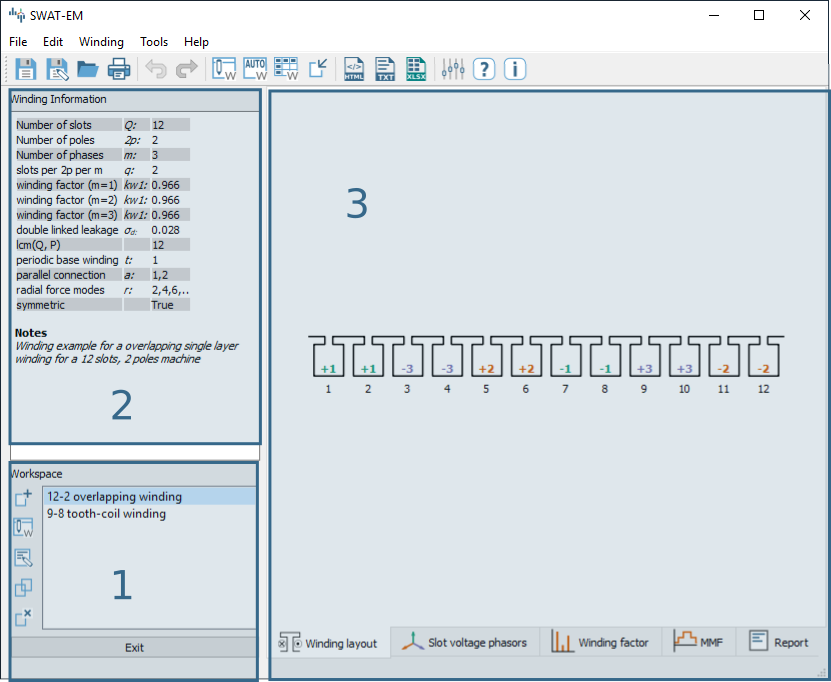
\includegraphics[width=0.99\textwidth,angle=0]{fig/mainwindow}
    \caption{Main-window}
    \label{fig:mainwindow}
\end{figure}
%
\section{Workspace}\label{sec:workspace}
A SWAT-EM project, that can be saved as *.wdg file can contain several different windings system.
So, one can define and compare these windings in the same window. The workspace shows all
the windings of the project. By clicking of the name all outputs (text and plots) gets updated.
The buttons on the left of (1) in figure \ref{fig:mainwindow} modifies the windings in the workspace
\begin{description}
 \item[New winding] Opens a dialog with all existing winding generator (see section \ref{sec:winding_generators}). 
		    One can choose any of these generators to create a winding layout.
 \item[Manual winding layout] Define the position of all coil sides by hand. (Not very comfortable
		    but full control)
 \item[Auto winding layout] Generates the winding automatically by number of slots, poles, ... (easy
                            to use, almost every symmetric winding is possible)
 \item[Winding table] Shows table slot/pole combinations (a good overview of possible combinations) 
 \item[Notes] If there a many windings in the project it might be a good idea to add some notes
              to the different layouts.
 \item[Clone] For modifying windings one can clone/duplicate an existing one. So a switch-back to the 
              initial state and a comparison is possible.
 \item[Delete] Deletes the selected winding.
\end{description}
%
While saving the project to file (File $\rightarrow$ save) all windings of the workspace are saved. 
\textbf{Note:} Renaming of windings is possible by double-click or by pressing F2 on keyboard.
%
%
\section{Winding information}
The text field (2) in figure \ref{fig:mainwindow} shows a summary of actual winding. 
%
\begin{center}
\begin{table}[h]
\begin{tabularx}{\textwidth}{lX}
$Q$ & Number of stator slots \\
$2p$ & Number of pole pairs  \\
$m$ & Number of phases \\
$q$ & Number of slots per pole per phase $q=\frac{Q}{2pm}$ \\
$kw1$ & Fundamental winding factor (for separate for each phase) \\
$lcm(Q,P)$ & Least common multiplier of number of slots an pole pairs. For permanent-magnet machines this is the first harmonic  number of the cogging torque \\
$t$ & Periodicity of the base winding. $t = gcd(Q, p)$ \\
$a$ & Number of possible parallel winding circuit. (In most cases a is equal to t) \\
$symmetric$ & True, if all phases are identically and shifted by a constant angle \\
$Notes$ & User defined description \\
\end{tabularx}
\end{table}
\end{center}


%
%
%
%
\section{Winding layout plot}
Many analyzing function results in plots which are shown on(3) in figure \ref{fig:mainwindow}.
Every plot has a toolbar on the bottom for zooming, panning and saving the figure to file.
%
%
\subsection{Winding layout}
The winding layout plot shows sketched slots and coil sides. The number and color defines the number
of phase the coil side belongs to. The sign (+ or -) defines the winding direction (+ means that the
wire goes into the plain and - out of the plain)
%
%
\subsection{Slot voltage phasors}
The impact of the coils can be represented by the star of slot. The theory behind this is
described in \cite{mueller1996berechnung} for example. Every coil side $S_i$ gets a phasor assigned with 
the angle 
\begin{align}
\alpha_i = \dfrac{2p \pi S_i}{Q}  \label{eqn:phasors_angle}
\end{align} 
%
The angle of the phasors can also be determined for the harmonics by adding the electrical ordinal
number $\nu_{el}$
\begin{align}
\alpha_{i,\nu} = \dfrac{2\nu p \pi S_i}{Q}  \label{eqn:phasors_angle2}
\end{align} 
%
% 
with $p$ pole pairs and the number of stator slots $Q$. If the coil side has a negative winding direction
$\pi$ is added to $alpha_i$ (turning down the phasor). With this the phasers $E_i$ can be generated
in the complex plain
%
\begin{align}
E_i = e^{j\alpha_i}
\end{align} 
%
All phasors of a phase are getting grouped a vectorial summed up which is shown as (1) in figure 
\ref{fig:phasors}. The dotted line represents the vectorial sum. The amplitude and the phase of
this is shown in (2).
%
\begin{figure}[htpb]
    \centering
    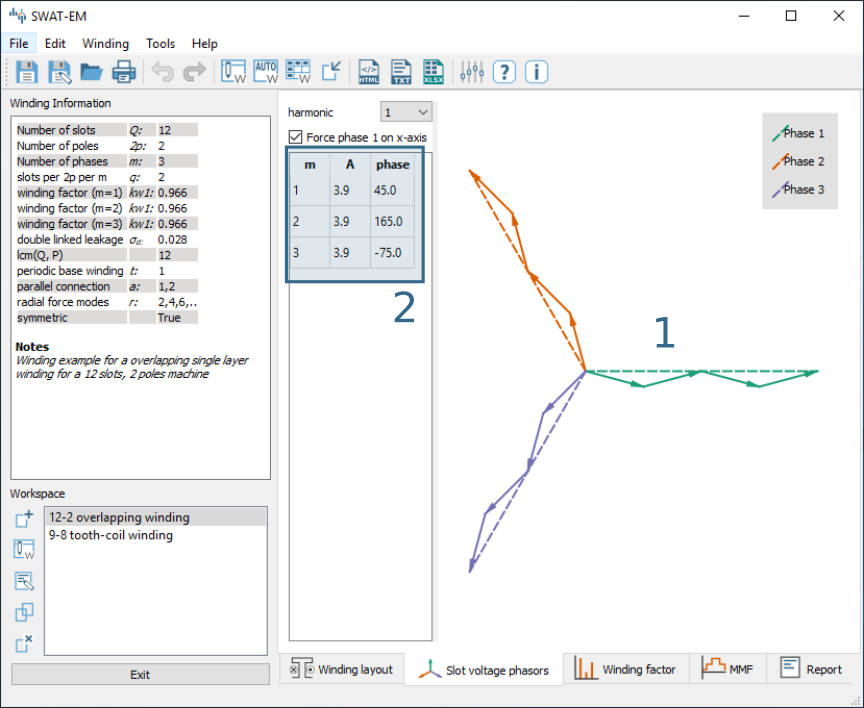
\includegraphics[width=0.99\textwidth,angle=0]{fig/mainwindow_phasors}
    \caption{Phasors plot}
    \label{fig:phasors}
\end{figure}
%
Options:
\begin{description}
 \item[harmonic] The star of slots can be drawn for any harmonic number by using \eqref{eqn:phasors_angle2}.
 \item[force phase 1 on x-axis] The angle of the sum of phasors depends on the location of the coil sides
                                in the slots. If the whole winding is shifted by some slots the winding is
                                still the same winding. However the phasors are getting a phase shift. To
                                compare different windings and for having an unified diagram one can set
                                this checkbox.
\end{description}
%
%
\FloatBarrier
\subsection{Winding factor}
The winding factor $k_w$ describes the coupling of the winding with the existing field in the stator. It depends
on the ordinal number $\nu$ (electrical or mechanical ordinal number possible). There are many methods for 
calculating the winding factor, for example from the MMF \ref{sec:MMF}. Unfortunately there are limitations
of this method because for three-phase windings the factor $k_{w3}$ can't be determined. Further calculation
methods derives specific equations based on the winding zones. However theses equation are not universal, so
there are many equations for different winding systems. To be general SWAT-EM uses the phasors of the
star of slots. The absolute value of the winding factor is defined by
%
\begin{align}
|k_{w}| = \frac{|\sum{E_i}|}{ \sum{| E_{i} |} }
\end{align} 
%
and for all harmonics with
%
\begin{align}
|k_{w,\nu}| = \frac{|\sum{E_{i,\nu}}|}{ \sum{| E_{i,\nu} |} }
\end{align} 
%
It can be seen in figure \ref{fig:phasors} that the winding factor gets the maximum value of 1 if all
phasors of a phase have the same phase angle. Typically the winding factor is specified with a sign. This
indicates the direction of the magnetic field wave, that is generated by the winding in the airgap. 
SWAT-EM determines the sign by generating the phasors plot for every harmonic number and detecting the
sequence of the phases. Figure \ref{fig:mainwindow_windingfactor} shows the values in (1) as a table
and the absolute values as a bar plot in (2).
%
\begin{figure}[htpb]
    \centering
    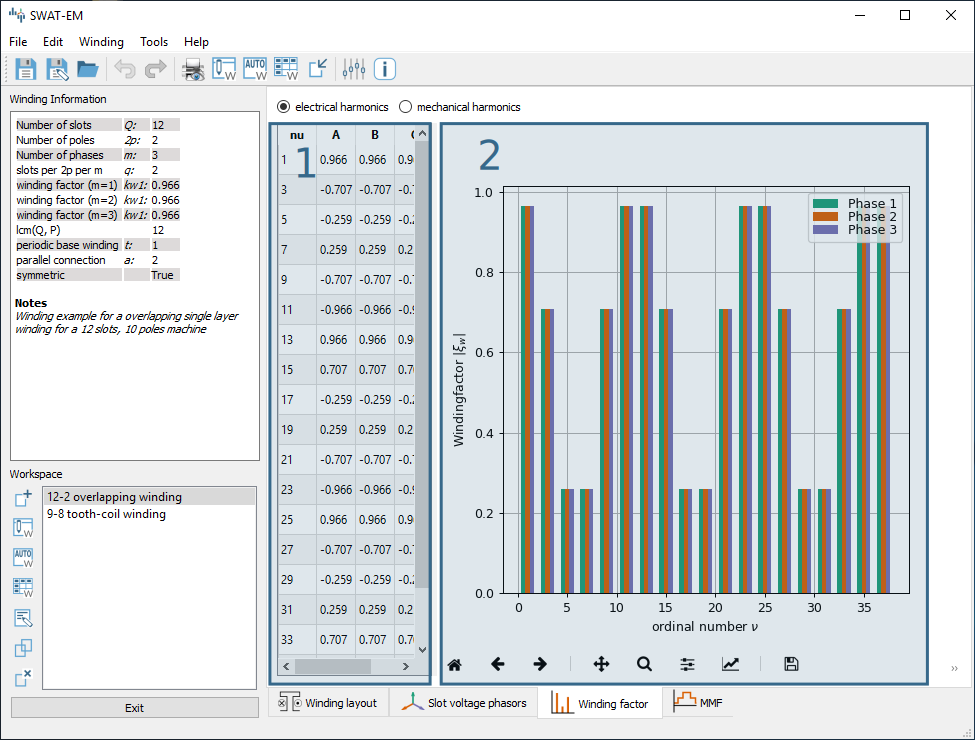
\includegraphics[width=0.99\textwidth,angle=0]{fig/mainwindow_windingfactor}
    \caption{Winding factor plot}
    \label{fig:mainwindow_windingfactor}
\end{figure}
%
Both can be displayed with respect to the mechanical $\nu$ or the electrical $\nu_{el}$ ordinal number by
the radio buttons on the top of the table.
\begin{description}
 \item[Mechanical harmonics] This representation is useful to detect all possible rotor pole numbers, which 
                             can be combined with the winding. Especially tooth-coil windings have many 
                             harmonics and so there are many pole-pairs per winding layout is possible. 
 \item[Electrical harmonics] If one have chosen a winding and a number of pole-pairs of the rotor it's
                             a good idea to switch to the electrical ordinal numbers. Here the numbers describes
                             influence of the winding of the waveform of the back-emf for permanent-magnet
                             machines for example. If the winding factor for the harmonics is low, the 
                             waveform is more sinusoidal.
\end{description}
%
%
\subsection{Magnetomotive force (MMF)} \label{sec:MMF}
For evaluation of the winding the so called "`Magnetomotive force"' or short MMF is a useful tool. It is
based on the the ampere-conductor distribution. This is shown for time $t=t_1$ with respect to the 
AC current system of $m$ phases.
%
\begin{figure}[htpb]
    \centering
    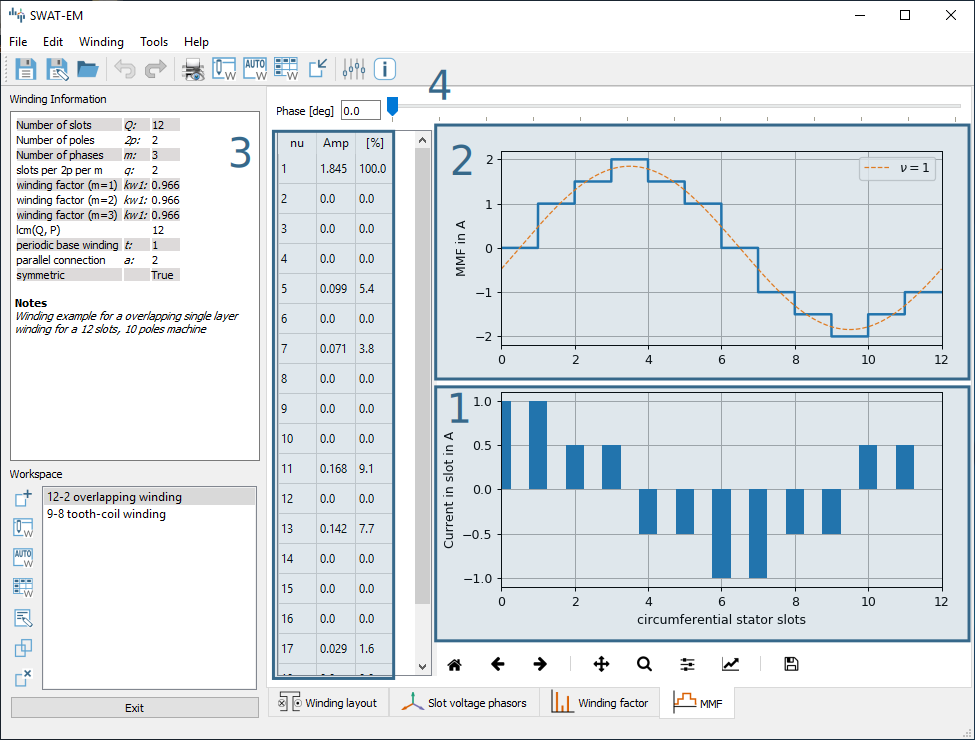
\includegraphics[width=0.99\textwidth,angle=0]{fig/mainwindow_MMF}
    \caption{Plot of the ampere-conductor distribution and the Magnetomotive force (MMF) }
    \label{fig:mainwindow_MMF}
\end{figure}
%
For every slot the winding direction ($d=\pm1$), number of turns $N_c$ the current $i$ gets summed up 
\begin{align}
\Theta_{slot} = \sum{d \cdot i N_c}.
\end{align} 
%
Therefor the distribution of ampere-turns is coupled with number of slots. (1) in Figure \ref{fig:mainwindow_MMF}
shows this for a winding example with $Q = 12$ slots, so there are 12 bars. In reality the distribution has
a width per bar which corresponds to the slot opening. However in theory (in this program) the distribution
can be interpreted as infinitely thin peaks. The integral of this leads to the MMF
\begin{align}
MMF(\alpha) = \int_0^{2\pi}{ \Theta d\alpha},
\end{align} 
%
which is shown in (2) in figure \ref{fig:mainwindow_MMF}.
The waveform of the MMF corresponds to the magnetic field, that is generated in the airgap by the winding.
For further information consider the literature (eg \cite{hendershot2010design}).
The plot also shows the fundamental and some of the harmonics. The number of harmonics which are plotted
can be defined relative to the fundamental. Please consider the "`Tools"' $\rightarrow$ "`Settings"' dialog.
The table (3) in the window displays the harmonic analyses of the MMF. With the slider (4) one can define
the phase angle of the AC current system for the MMF plot. Note that the phase angle has no effect on
the harmonic content of the MMF, so the harmonic analyses is independent from it.
%
%
%
\section{Winding Generators}\label{sec:winding_generators}
SWAT-EM comes with many different winding generators. Each of them have different features.
%
%
\subsection{Manual layout}\label{sec:manual_generator}
%
The manual layout generator (figure \ref{fig:manual_layout_dialog} ) is the most basic generator in SWAT-EM. 
One can define the position and the number of turns for each coil side by hand. With this every winding layout 
can be sketched and analyzed. The price of this is the comparatively large manual effort.
%
\begin{figure}[htpb]
    \centering
    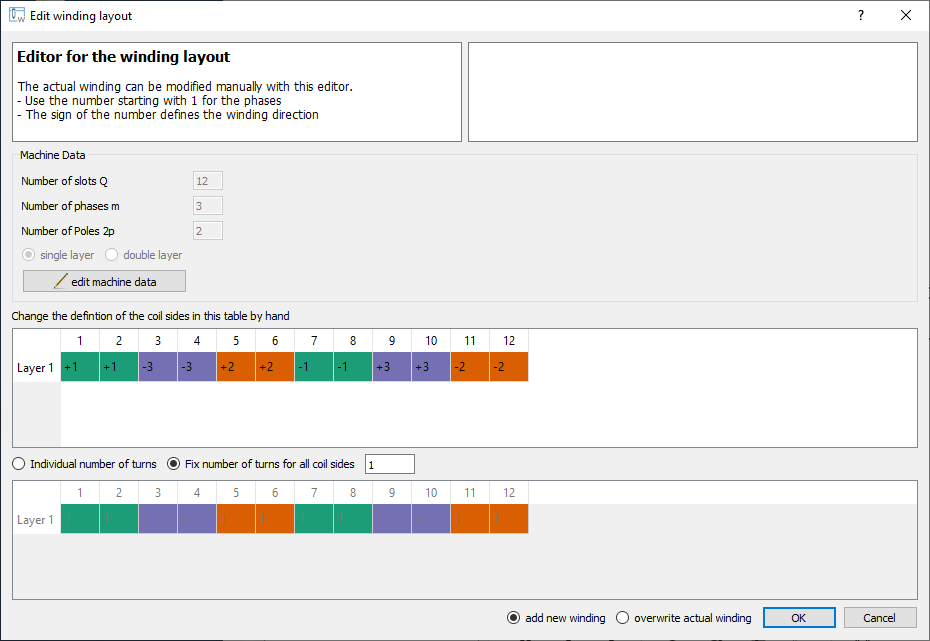
\includegraphics[width=0.99\textwidth,angle=0]{fig/manual_layout}
    \caption{Manual winding generator }
    \label{fig:manual_layout_dialog}
\end{figure}
%
\begin{description}
 \item[Button "`edit machine data"'] Use this dialog if you want to change the number of slots $Q$,
          of phases $m$, of poles $2p$ or layers.
 \item[definition of the coil sides] Use the table to define the phase for the layers in each slot.
          The number describes the phase number. The color is added automatically for overview. The 
          sign defines the winding direction (+ into the plane, - out of the plane)
 \item[number of turns] If radio button is set to "`fix number of turns for all coil sides"' one can
          type the number of turns in the edit field apart from that. While choosing "`individual
          number of turns"' one can define this for each coil side. Use the table below 
 \item[info] On the upper right there is an info field. While the user defines the winding there is
          a live-analysis. If there is an unsymmetrical winding or if the sum of all winding turns is not 
          zero for example, the user get an info.
 \item[overwrite winding] There are two different possible action while exiting an generator dialog with
          the ok button. If the radio button "`add new winding"' is selected, the winding in the generator
          winding is added to the workspace in the main window. If "`overwrite"' is selected, than the 
          actual selected winding of the workspace getting overwritten. Be relaxed, if you have overwritten
          your winding accidentally, there is an undo function in the main window.
\end{description}
%
%
\FloatBarrier
\subsection{Automatic layout}\label{sec:automatic_generator}
With the automatic winding generator it is possible to generate almost every symmetric winding system, 
except "`dead coil windings"' (where some slots are empty). 
This includes
\begin{itemize}
 \item overlapping full pitch winding
 \item overlapping fractional slot winding
 \item tooth coil winding
 \item all above as single-layer or double-layer
\end{itemize}
%
This generator uses the star of slots to for defining
the coil sides in the slots, based on the theory of \cite{1629527}.
%
\begin{figure}[htpb]
    \centering
    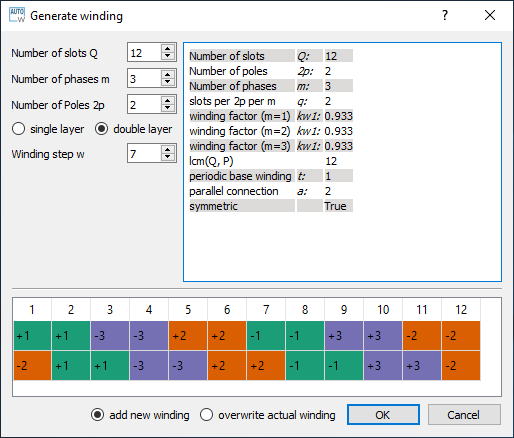
\includegraphics[width=0.80\textwidth,angle=0]{fig/auto_winding}
    \caption{Automatic winding generator }
    \label{fig:auto_winding}
\end{figure}
%
%
\begin{description}
 \item[Machine data] Number of slots $Q$, phases $m$ and poles $2p$ 
 \item[layer] Double layer winding means, that in every slot there are two coil sides (from the same
      or from different phases)
 \item[winding step] Every coil has an "`in"' and an "`out"' conductor, which are connected via 
       the winding overhang. The winding step defines the distance between "`in"' and "`out"' in slots.
       If winding-step is 1 a tooth-coil winding will be created. Note: For single layer windings 
       there are some restriction to accommodate all coil sides, so in this case the winding step
       can't be influenced.       
 \item[overwrite winding] There are two different possible action while exiting an generator dialog with
          the ok button. If the radio button "`add new winding"' is selected, the winding in the generator
          winding is added to the workspace in the main window. If "`overwrite"' is selected, than the 
          actual selected winding of the workspace getting overwritten. Be relaxed, if you have overwritten
          your winding accidentally, there is an undo function in the main window.
 \item[layout table] The lower table shows the actual defined winding. Note, that layout can't changed here
          by hand. If you want to change, than accept the winding with OK to the workspace in the main window
          and use the manual generator (section \ref{sec:manual_generator}). The winding will be transmitted.
\end{description}
%
%
\FloatBarrier
\subsection{Winding table}
%
This generator gives an overview about possible slot/poles combinations. So it's generator
with a broad but not very deep view on windings. It can be useful
in the early state of designing electrical machine, for example to define the appropriate
number of slots and poles.

While clicking on a item in the upper
table, the winding characteristics shown on the left side and the winding layout is
shown on the bottom table. As with the other generators the selected winding can be transferred to the workspace in the main window.

For some slot/pole combinations there
are many winding system possible where this generator shows the winding with the highest
fundamental winding factor $k_{w,1}$. At this time there is no way to modify the windings
(changing winding steps for example). For more control you have to use other generators like
\ref{sec:manual_generator} or \ref{sec:automatic_generator}.
%
\begin{figure}[htpb]
    \centering
    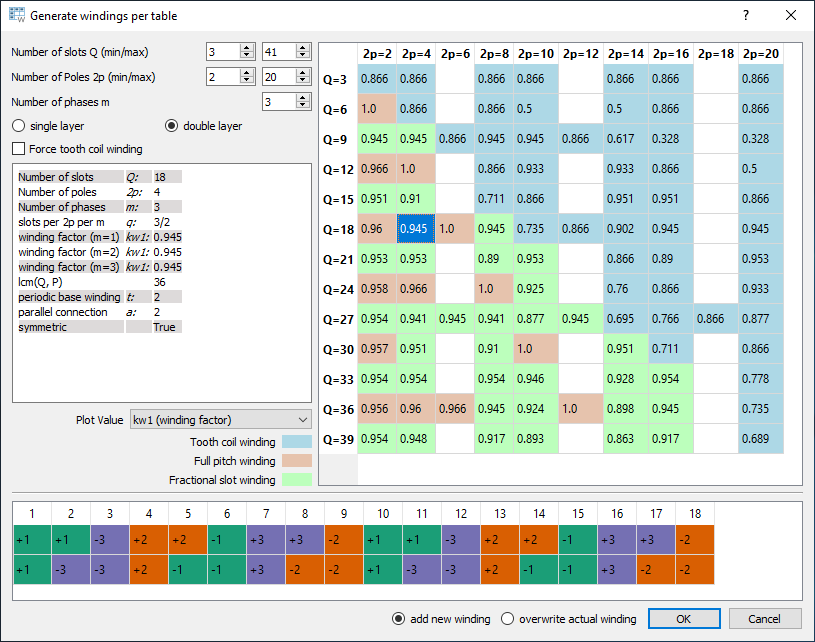
\includegraphics[width=0.99\textwidth,angle=0]{fig/winding_table}
    \caption{Table of possible windings for diffrent slot/pole combinations }
    \label{fig:winding_table}
\end{figure}
%
%
\begin{description}
 \item[Number of slots] Defines the range of number the number of slots $Q$ for them
        table. For symmetric windings the number of slots must be a integer multiple 
        of the number of phases $m$.
        \begin{align}
        Q = k \cdot m, \text{ with }k = 1, 2, 3...
        \end{align} 
        For single layer windings (without dead coil windings) the number of slots must be doubled
        \begin{align}
        Q = 2 \cdot k \cdot m, \text{ with }k = 1, 2, 3...
        \end{align} 
 \item[Number of poles] The number of poles $2p$. Only even integer values $\geq2$ are valid.
 \item[Number of phases] The number of phases $m$ in the machine. Every integer value $>1$ is valid.
 \item[layers] Defines the number of layers for the table. At this time only single layer and
        double layer windings are possible.
 \item[Force tooth coil winding] In some cases you may want to realize tooth coil windings, 
        even when the winding factor isn't very high. In this case  the winding step is set to $w=1$. 
 \item[plot value] Defines the number which is shown in the upper table.
    \begin{description}
    \item[kw1] The fundamental winding factor. A big number (near to ``1'') means a high-torque.
    \item[q] The number of slots $Q$ per pole $2p$ per phase $m$. It characterized the winding system.
            \begin{align}
            p = \frac{Q}{2p\cdot m}
            \end{align} 
    
    \item[t] The number of the periodic sequence of identical ``base-'' windings. 
    \item[a] The number of possible parallel circuits of coil groups in the winding. In most 
            cases it`s the same as $t$. But for some windings it`s possible to connect
            coil groups in parallel while changing the start and end of the coils.
    \item[lcm(Q,2p)] Means the least common multiple of the number of slots $Q$ and number
            of poles $2p$. For permanent-magnet machines this is the first ordinal
            number of the cogging torque. Tends to be true: The higher the ordinal number the lower the amplitude of the cogging torque.
    \end{description}
  \item[overwrite winding] There are two different possible action while exiting an generator dialog with
          the OK button. If the radio button "`add new winding"' is selected, the winding in the generator
          winding is added to the workspace in the main window. If "`overwrite"' is selected, than the 
          actual selected winding of the workspace getting overwritten. Be relaxed, if you have overwritten
          your winding accidentally, there is an undo function in the main window.
\end{description}
%
%
%
\section{Import winding}
As in \ref{sec:workspace} described you can have many winding system in the workspace.
In some cases you may want to have a winding in your workspace which is saved as a
*.wdg file on the hard disk. This can be done by the import function.
%
\begin{figure}[htpb]
    \centering
    
\includegraphics[width=0.8\textwidth,angle=0]{fig/import}
    \caption{Import winding from file }
    \label{fig:import}
\end{figure}
%
For import a window opens with the file dialog. Navigate to an existing *.wdg file. After that you get a list of all windings systems of the file (figure \ref{fig:import}). Choose
all windings you want to import into the workspace.






\bibliographystyle{unsrt}
\bibliography{literature}

\end{document}







